\section{Extending and contributing to \aspect}
\label{sec:extending}

\aspect{} is designed to be an extensible code. In particular, it
uses both a plugin architecture and a set of signals through which it is
trivial to replace or extend certain components of the program. Examples of
things that are simple to extend are:
\begin{itemize}
\item the material description,
\item the geometry,
\item the gravity description,
\item the initial conditions,
\item the boundary conditions,
\item the functions that postprocess the solution, i.e., that can compute
  derived quantities such as heat fluxes over part of the boundary, mean
  velocities, etc.,
\item the functions that generate derived quantities that can be put into
  graphical output files for visualization such as fields that depict the
  strength of the friction heating term, spatially dependent actual
  viscosities, and so on,
\item the computation of refinement indicators,
\item the determination of how long a computation should run.
\end{itemize}
This list may also have grown since this section was written.
We will discuss the way this is achieved in Sections~\ref{sec:plugins} and
\ref{sec:plugins-concrete}. Changing the core functionality, i.e., the basic equations
\eqref{eq:stokes-1}--\eqref{eq:temperature}, and how they are solved is
arguably more involved. We will discuss this in Section
\ref{sec:extending-solver}.

\note{The purpose of coming up with ways to make extensibility simple is that if
you want to extend \aspect{} for your own purposes, you can do this in a
separate set of files that describe your situation, rather than by modifying
the \aspect{} source files themselves. This is important, because (i) it makes
it possible for you to update \aspect{} itself to a newer version without
losing the functionality you added (because you did not make any changes to
the \aspect{} files themselves), (ii) because it makes it possible to keep
unrelated changes separate in your own set of files, in a place where they are
simple to find, and (iii) because it makes it much easier for you to share
your modifications and additions with others.}

Since \aspect{} is written in C++ using the \dealii{} library, you
will have to be proficient in C++. You will also likely have
to familiarize yourself with this library for which there is an extensive
amount of documentation:
\begin{itemize}
\item The manual at
  \url{https://www.dealii.org/developer/doxygen/deal.II/index.html} that
  describes in detail what every class, function and variable in \dealii{}
  does.
\item A collection of modules at
  \url{https://www.dealii.org/developer/doxygen/deal.II/modules.html} that give
  an overview of whole groups of classes and functions and how they work
  together to achieve their goal.
\item The \dealii{} tutorial at
  \url{https://www.dealii.org/developer/doxygen/tutorial/index.html} that
  provides a step-by-step introduction to the library using a sequence of
  several dozen programs that introduce gradually more complex topics. In
  particular, you will learn \dealii's way of \textit{dimension independent
  programming} that allows you to write the program once, test it in 2d, and
  run the exact same code in 3d without having to debug it a second time.
\item The step-31 and step-32 tutorial programs at
  \url{https://www.dealii.org/developer/doxygen/deal.II/step_31.html} and
  \url{https://www.dealii.org/developer/doxygen/deal.II/step_32.html} from
  which \aspect{} directly descends.
\item An overview of many general approaches to numerical methods, but also
  a discussion of \dealii{} and tools we use in programming, debugging and
  visualizing data are given in Wolfgang Bangerth's video lectures. These
  are linked from the \dealii{} website at \url{https://www.dealii.org/}
  and directly available at
  \url{http://www.math.tamu.edu/~bangerth/videos.html}.
\item The \dealii{} Frequently Asked Questions at
  \url{https://github.com/dealii/dealii/wiki/Frequently-Asked-Questions}
  that also have extensive sections on developing code with \dealii{} as well
  as on debugging. It also answers a number of questions we frequently get
  about the use of C++ in \dealii{}.
\item Several other parts of the \dealii{} website at
  \url{https://www.dealii.org/} also have information that may be relevant if
  you dive deeper into developing code. If you have questions, the mailing
  lists at \url{https://www.dealii.org/mail.html} are also of general help.
\item A general overview of \dealii{} is also provided in the paper
  \cite{BHK07}.
\end{itemize}

As a general note, by default \aspect{} utilizes a \dealii{} feature called \textit{debug
  mode}, see also the introduction to this topic in
Section~\ref{sec:debug-mode}. If you develop code, you will definitely want
this feature to be on, as it will capture the vast majority of bugs you
will invariably introduce in your code.

When you write new functionality and run
the code for the first time, you will almost invariably first have to deal
with a number of these assertions that point out problems in your code. While
this may be annoying at first, remember that these are actual bugs in your
code that have to be fixed anyway and that are much easier to find if the
program aborts than if you have to go by their more indirect results such as
wrong answers. The Frequently Asked Questions at
\url{https://github.com/dealii/dealii/wiki/Frequently-Asked-Questions}
contain a section on how to debug \dealii{} programs.

The downside of debug mode, as mentioned before, is that it makes the program
much slower. Consequently, once you are
confident that your program actually does what it is intended to do --
\textbf{but no earlier!} --, you may want to switch to optimized mode that
links \aspect{} with a version of the \dealii{} libraries that uses compiler
optimizations and that does not contain the \texttt{assert} statements
discussed above. This switch can be facilitated by editing the top of the
\aspect{} \url{Makefile} and recompiling the program.

In addition to these general comments, \aspect{} is itself extensively
documented. You can find documentation on all classes, functions and
namespaces starting from the \url{doc/doxygen/index.html} page.


\subsection{The idea of plugins and the \texttt{SimulatorAccess} and \texttt{Introspection} classes}
\label{sec:plugins}

The most common modification you will probably want to do to \aspect{} are to
switch to a different material model (i.e., have different values of
functional dependencies for the coefficients $\eta,\rho,C_p, \ldots$ discussed
in Section~\ref{sec:coefficients}); change the geometry; change the direction
and magnitude of the gravity vector $\mathbf g$; or change the initial and
boundary conditions.

To make this as simple as possible, all of these parts of the program (and some more) have
been separated into what we call \textit{plugins} that can be replaced quickly
and where it is simple to add a new implementation and make it available to the rest of the
program and the input parameter file. There are \textit{a lot} of plugins
already, see Fig.~\ref{fig:plugins}, that will often be useful starting points
and examples if you want to implement plugins yourself.

\begin{figure}[tbp]
  \centering
  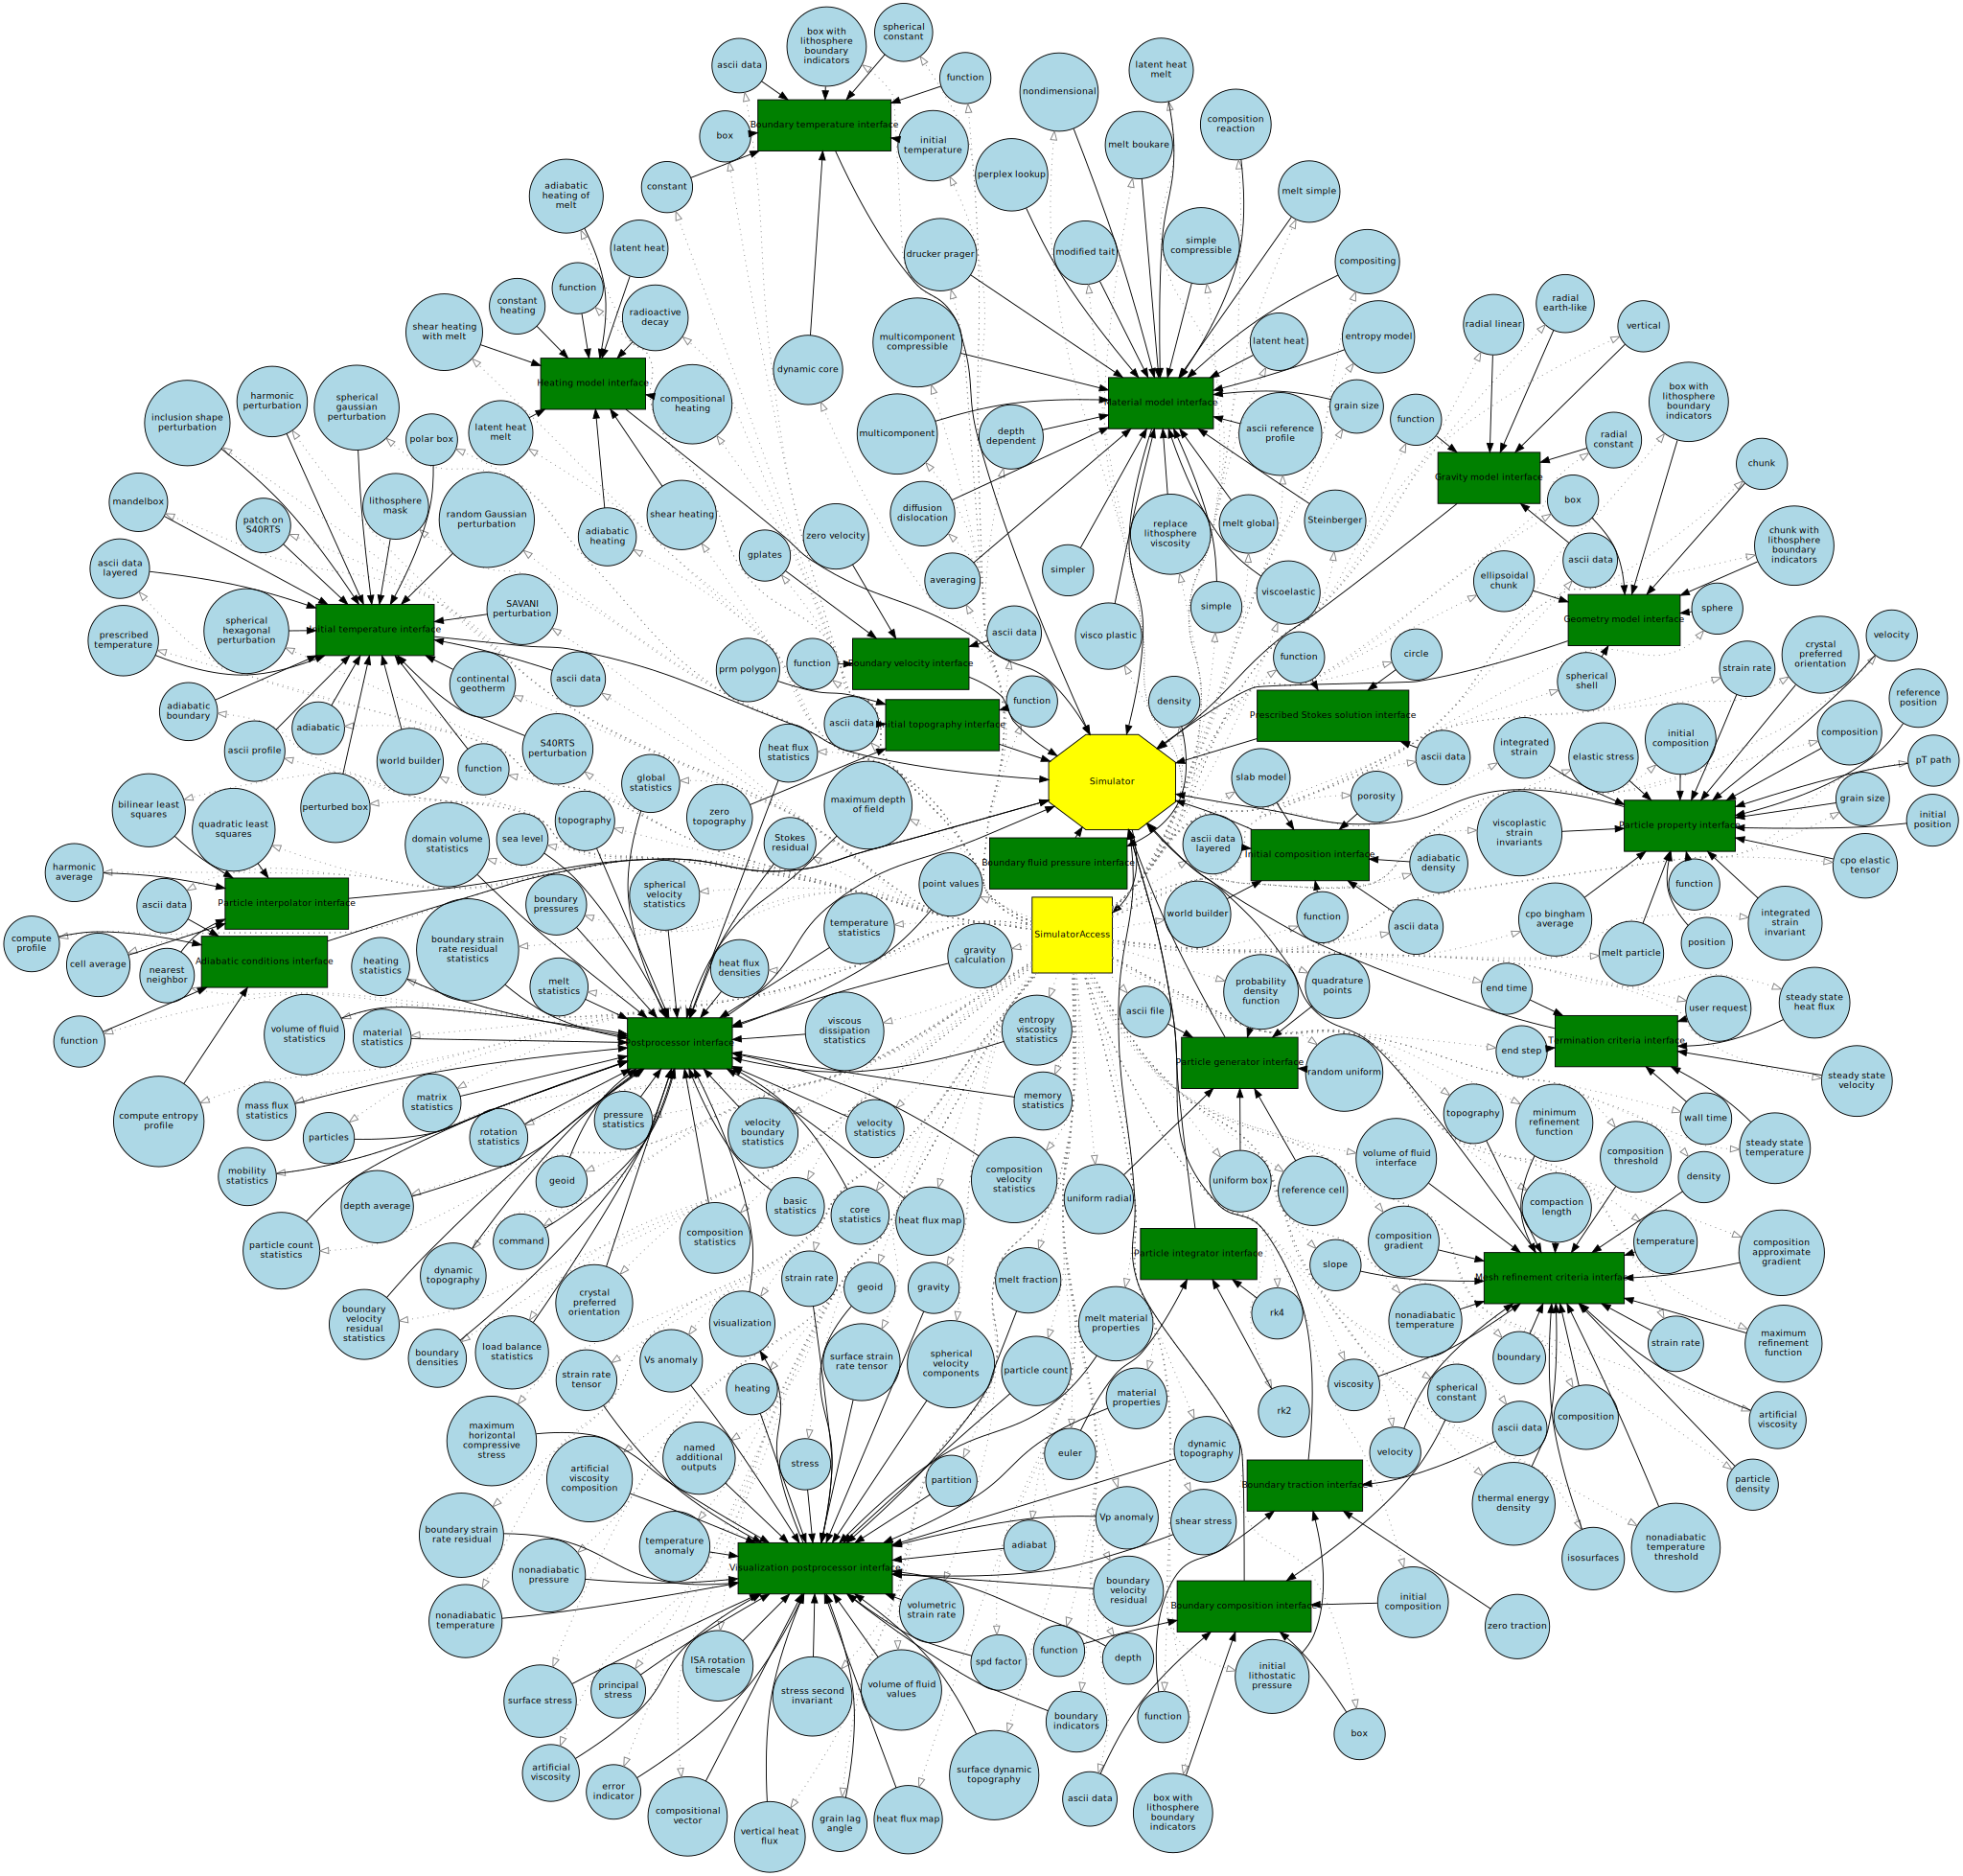
\includegraphics[width=0.95\textwidth]{plugin_graph.pdf}
  \caption{\it The graph of all current plugins of \aspect{}. The yellow
  octagon and square represent the \texttt{Simulator} and
  \texttt{SimulatorAccess} classes. The green boxes are interface classes for
  everything that can be changed by plugins. Blue circles correspond to plugins
  that implement particular behavior. The graph is of course too large to allow
  reading individual plugin names (unless you zoom far into the page), but is
  intended to illustrate the architecture of \aspect{}.}
  \label{fig:plugins}
\end{figure}

The way this is achieved is through the
following two steps:
\begin{itemize}
\item The core of \aspect{} really only communicates with material models,
  geometry descriptions, etc., through a simple and very basic
  interface. These interfaces are declared in the
  \url{include/aspect/material_model/interface.h},
  \url{include/aspect/geometry_model/interface.h}, etc., header files. These
  classes are always called \texttt{Interface}, are located in namespaces that
  identify their purpose, and their documentation can be found from the
  general class overview in \url{doc/doxygen/classes.html}.

  To show an example of a rather minimal case, here is the declaration of the
\href{doc/doxygen/classaspect_1_1GravityModel_1_1Interface.html}{aspect::GravityModel::Interface} class (documentation comments have
  been removed):
  \begin{lstlisting}[frame=single,language=C++]
    class Interface
    {
      public:
        virtual ~Interface();

        virtual
        Tensor<1,dim>
        gravity_vector (const Point<dim> &position) const = 0;

        static void declare_parameters (ParameterHandler &prm);

        virtual void parse_parameters (ParameterHandler &prm);
    };
  \end{lstlisting}

  If you want to implement a new model for gravity, you just need to write a
  class that derives from this base class and implements the
  \texttt{gravity\_vector} function. If your model wants to read parameters
  from the input file, you also need to have functions called
  \texttt{declare\_parameters} and \texttt{parse\_parameters} in your class
  with the same signatures as the ones above. On the other hand, if the new
  model does not need any run-time parameters, you do not need to overload
  these functions.%
  \footnote{At first glance one may think that only the
    \texttt{parse\_parameters} function can be overloaded since
    \texttt{declare\_parameters} is not virtual. However, while the latter is
    called by the class that manages plugins through pointers to the interface
    class, the former function is called essentially at the time of
    registering a plugin, from code that knows the actual type and name of the
    class you are implementing. Thus, it can call the function -- if it exists
    in your class, or the default implementation in the base class if it doesn't
    -- even without it being declared as virtual.}

  Each of the categories above that allow plugins have several implementations
  of their respective interfaces that you can use to get an idea of how to
  implement a new model.

\item At the end of the file where you implement your new model, you need to
  have a call to the macro \texttt{ASPECT\_REGISTER\_GRAVITY\_MODEL} (or the
  equivalent for the other kinds of plugins). For
  example, let us say that you had implemented a gravity model that takes
  actual gravimetric readings from the GRACE satellites into account, and had
  put everything that is necessary into a class
  \texttt{aspect::GravityModel::GRACE}. Then you need a statement like this at
  the bottom of the file:
  \begin{lstlisting}[frame=single,language=C++]
    ASPECT_REGISTER_GRAVITY_MODEL
    (GRACE,
     "grace",
     "A gravity model derived from GRACE "
     "data. Run-time parameters are read from the parameter "
     "file in subsection 'Radial constant'.");
  \end{lstlisting}
  Here, the first argument to the macro is the name of the class. The second
  is the name by which this model can be selected in the parameter file. And
  the third one is a documentation string that describes the purpose of the
  class (see, for example, Section~\ref{parameters:Gravity_20model} for an
  example of how existing models describe themselves).

  This little piece of code ensures several things: (i) That the parameters
  this class declares are known when reading the parameter file. (ii) That you
  can select this model (by the name ``grace'') via the run-time parameter
  \texttt{Gravity model/Model name}. (iii) That \aspect{} can create an object
  of this kind when selected in the parameter file.

  Note that you need not announce the existence of this class in any other
  part of the code: Everything should just work automatically.%
  \footnote{The existing implementations of models of the gravity and other interfaces
  declare the class in a header file and define the member functions in a
  \texttt{.cc} file. This is done so that these classes show up in our
  doxygen-generated documentation, but it is not necessary: you can put your
  entire class declaration and implementation into a single file as long as
  you call the macro discussed above on it. This single file is all you need
  to touch to add a new model.}
  This has the advantage that things are neatly separated: You do not need to
  understand the core of \aspect{} to be able to add a new gravity model that
  can then be selected in an input file. In fact, this is true for
  all of the plugins we have: by and large, they just receive some data
  from the simulator and do something with it (e.g., postprocessors), or they
  just provide information (e.g., initial meshes, gravity models), but their
  writing does not require that you have a fundamental understanding
  of what the core of the program does.
\end{itemize}

The procedure for the other areas where plugins are supported works
essentially the same, with the obvious change in namespace for the interface
class and macro name.

In the following, we will discuss the requirements for individual plugins. Before
doing so, however, let us discuss ways in which plugins can query other
information, in particular about the current state of the simulation.
To this end, let us not consider those plugins that by and large just
provide information without any context of the simulation, such as gravity models,
prescribed boundary velocities, or initial temperatures. Rather, let us
consider things like postprocessors that can compute things like boundary heat
fluxes. Taking this as an example (see Section~\ref{sec:postprocessors}), you are
required to write a function with the following interface
\begin{lstlisting}[frame=single,language=C++]
    template <int dim>
    class MyPostprocessor : public aspect::Postprocess::Interface
    {
      public:
        virtual
        std::pair<std::string,std::string>
        execute (TableHandler &statistics);

      // ... more things ...
\end{lstlisting}
The idea is that in the implementation of the \texttt{execute} function
you would compute whatever you are interested in (e.g., heat fluxes)
and return this information in the statistics object that then gets written
to a file (see Sections~\ref{sec:running-overview} and \ref{sec:viz-stat}).
A postprocessor may also generate other files if it so likes -- e.g., graphical
output, a file that stores the locations of particles, etc.
To do so, obviously you need access to the current solution. This is
stored in a vector somewhere in the core of \aspect{}. However, this
vector is, by itself, not sufficient: you also need to know the finite
element space it is associated with, and for that the triangulation it
is defined on. Furthermore, you may need to know what the current
simulation time is. A variety of other pieces of information enters
computations in these kinds of plugins.

All of this information is of course part of the core of \aspect{},
as part of the
\href{doc/doxygen/classaspect_1_1Simulator.html}{aspect::Simulator
class}. However, this is a rather heavy class: it's got dozens of
member variables and functions, and it is the one that does all
of the numerical heavy lifting. Furthermore, to access data in
this class would require that you need to learn about the internals,
the data structures, and the design of this class.
It would be poor design if plugins had to access information from this
core class directly. Rather, the way this works is that those plugin
classes that wish to access information about the state of the simulation
inherit from the
\href{doc/doxygen/classaspect_1_1SimulatorAccess.html}{aspect::SimulatorAccess
class}. This class has an interface that looks like this:
\begin{lstlisting}[frame=single,language=C++]
    template <int dim>
    class SimulatorAccess
    {
    protected:
      double       get_time () const;

      std::string  get_output_directory () const;

      const LinearAlgebra::BlockVector &
      get_solution () const;

      const DoFHandler<dim> &
      get_dof_handler () const;

      // ... many more things ...
\end{lstlisting}
This way, \href{doc/doxygen/classaspect_1_1SimulatorAccess.html}{SimulatorAccess} makes information available to plugins
without the need for them to understand details of the core of \aspect{}.
Rather, if the core changes, the \href{doc/doxygen/classaspect_1_1SimulatorAccess.html}{SimulatorAccess} class can still
provide exactly the same interface. Thus, it insulates plugins from having
to know the core. Equally importantly, since \href{doc/doxygen/classaspect_1_1SimulatorAccess.html}{SimulatorAccess} only
offers its information in a read-only way it insulates the core from
plugins since they can not interfere in the workings of the core except
through the interface they themselves provide to the core.

Using this class, if a plugin class \texttt{MyPostprocess} is then not only
derived from the corresponding \texttt{Interface} class but \textit{also}
from the \href{doc/doxygen/classaspect_1_1SimulatorAccess.html}{SimulatorAccess}
class (as indeed most plugins are, see the dashed arrows in
Fig.~\ref{fig:plugins}), then you can write a member function of the following
kind (a nonsensical but instructive example; see Section~\ref{sec:postprocessors} for more details on what postprocessors do and how they are implemented):%
\footnote{For complicated, technical reasons, in the code below we need to
  access elements of the \href{doc/doxygen/classaspect_1_1SimulatorAccess.html}{SimulatorAccess} class using the notation
  \texttt{this->get\_solution()}, etc. This is due to the fact that both the
  current class and the base class are templates. A long description of
  why it is necessary to use \texttt{this->} can be found in the \dealii{}
  Frequently Asked Questions.}
\begin{lstlisting}[frame=single,language=C++]
    template <int dim>
    std::pair<std::string,std::string>
    MyPostprocessor<dim>::execute (TableHandler &statistics)
    {
      // compute the mean value of vector component 'dim' of the solution
      // (which here is the pressure block) using a deal.II function:
      const double
        average_pressure = VectorTools::compute_mean_value (this->get_mapping(),
                                                            this->get_dof_handler(),
                                                            QGauss<dim>(2),
                                                            this->get_solution(),
                                                            dim);
      statistics.add_value ("Average pressure", average_pressure);

      // return that there is nothing to print to screen (a useful
      // plugin would produce something more elaborate here):
      return std::pair<std::string,std::string>();
    }
\end{lstlisting}

The second piece of information that plugins can use is called ``introspection''.
In the code snippet above, we had to use that the pressure variable is at
position \texttt{dim}. This kind of \textit{implicit knowledge} is usually
bad style: it is error prone because one can easily forget where each
component is located; and it is an obstacle to the extensibility of a code
if this kind of knowledge is scattered all across the code base.

Introspection is a way out of this dilemma. Using the \texttt{SimulatorAccess::introspection()}
function returns a reference to an object (of type
\href{doc/doxygen/structaspect_1_1Introspection.html}{aspect::Introspection})
that plugins can use to learn about these sort of conventions. For example,
\texttt{this->introspection().component\_mask.pressure} returns a
component mask (a deal.II concept that describes a list of booleans for each
component in a finite element that
are true if a component is part of a variable we would like to select and
false otherwise) that describes which component of the finite element
corresponds to the pressure. The variable, \texttt{dim}, we need above
to indicate that we want the pressure component can be accessed
as \texttt{this->introspection().component\_indices.pressure}. While this
is certainly not shorter than just writing \texttt{dim}, it may in
fact be easier to remember. It is most definitely less prone to
errors and makes it simpler to extend the code in the future because
we don't litter the sources with ``magic constants'' like the one
above.

This \href{doc/doxygen/structaspect_1_1Introspection.html}{aspect::Introspection} class
has a significant number of variables that can be used in this way, i.e.,
they provide symbolic names for things one frequently has to do and
that would otherwise require implicit knowledge of things such as the
order of variables, etc.


\subsection{How to write a plugin}
\label{sec:write-plugin}

Before discussing what each kind of plugin actually has to implement (see the
next subsection), let us briefly go over what you actually have to do when
implementing a new plugin. Essentially, the following steps are all you need to
do:
\begin{itemize}
  \item Create a file, say \texttt{my\_plugin.cc} that contains the declaration
  of the class you want to implement. This class must be derived from one of the
  \texttt{Interface} classes we will discuss below. The file also needs to
  contain the implementation of all member functions of your class.

  As discussed above, it is possible -- but not necessary -- to split this file
  into two: a header file, say \texttt{my\_plugin.h}, and the
  \texttt{my\_plugin.cc} file (or, if you prefer, into multiple source files).
  We do this for all the existing plugins in \aspect{} so that the documentation
  of these plugins shows up in the
  doxygen-generated documentation. However, for your own plugins, there is
  typically no need for this split. The only occasion where this would be useful
  is if some plugin actually makes use of a different plugin (e.g., the
  implementation of a gravity model of your own may want to query some
  specifics of a geometry model you also implemented); in that case the
  \textit{using} plugin needs to be able to see the declaration of the class of
  the \textit{used} plugin, and for this you will need to put the declaration of
  the latter into a header file.

  \item At the bottom of the \texttt{my\_plugin.cc} file, put a statement that
  instantiates the plugin, documents it, and makes it available to the parameter
  file handlers by registering it. This is always done using one of the
  \texttt{ASPECT\_REGISTER\_*} macros that will be discussed in the next
  subsections; take a look at how they are used in the existing plugins in the
  \aspect{} source files.

  \item You need to compile the file. There are two ways by which this can be
  achieved:
  \begin{itemize}
    \item Put the \texttt{my\_plugin.cc} into one of the \aspect{} source
    directories and call \texttt{cmake .} followed by \texttt{make} to ensure
    that it actually gets compiled. This approach has the advantage that you do
    not need to worry much about how the file actually gets compiled. On the
    other hand, every time you modify the file, calling \texttt{make} requires
    not only compiling this one file, but also link \aspect{}. Furthermore, when
    you upgrade from one version of \aspect{} to another, you need to remember
    to copy the \texttt{my\_plugin.cc} file.

    \item Put the  \texttt{my\_plugin.cc} file into a directory of your choice
    and compile it into a shared library yourself. This may be as easy as
    calling
    \begin{verbatim}
 g++ -I/path/to/aspect/headers -I/path/to/deal.II/headers \
     -fPIC -shared my_plugin.cc -o my_plugin.so
    \end{verbatim}
    on Linux, but the command may be different on other systems. Now you only
    need to tell \aspect{} to load this shared library at startup so that the
    plugin becomes available at run time and can be selected from the input
    parameter file. This is done using the \texttt{Additional shared libraries}
    \index[prmindex]{Additional shared libraries}
    \index[prmindexfull]{Additional shared libraries}
    parameter in the input file, see Section~\ref{parameters:global}. This
    approach has the upside that you can keep all files that define new plugins
    in your own directories where you also run the simulations, also making it
    easier to keep around your plugins as you upgrade your \aspect{}
    installation. On the other hand, compiling the file into a shared library is
    a bit more that you need to do yourself. Nevertheless, this is the preferred
    approach.

    In practice, the compiler line above can become tedious because it includes
    paths to the \aspect{} and \dealii{} header files, but possibly also other
    things such as Trilinos headers, etc. Having to remember all of these pieces
    is a hassle, and a much easier way is in fact to set up a mini-CMake project
    for this. To this end, simply copy the file \url{doc/plugin-CMakeLists.txt}
    to the directory where you have your plugin source files and rename it to
    \texttt{CMakeLists.txt}.
  \end{itemize}
  You can then just run the commands
    \begin{verbatim}
 cmake -DAspect_DIR=/path/to/aspect .
 make
    \end{verbatim}
    and it should compile your plugin files into a shared library
    \texttt{my\_plugin.so}. A concrete example of this process is discussed in
    Section~\ref{sec:benchmark-run}. Of course, you may want to choose different names
    for the source files \texttt{source\_1.cc}, \texttt{source\_2.cc} or the name of
    the plugin \texttt{my\_plugin}.

    In essence, what these few lines do is that they find an \aspect{}
    installation (i.e., the directory where you configured and compiled it,
    which may be the same directory as where you keep your sources, or a
    different one, as discussed in Section~\ref{sec:installation}) in either the
    directory explicitly specified in the \texttt{Aspect\_DIR} variable passed
    to \texttt{cmake}, the shell environment variable \texttt{ASPECT\_DIR}, or just one directory up. It then
    sets up compiler paths and similar, and the following lines simply define
    the name of a plugin, list the source files for it, and define everything
    that's necessary to compile them into a shared library. Calling
    \texttt{make} on the command line then simply compiles everything.
\end{itemize}

\note{Complex projects built on \aspect{} often require plugins of more than
just one kind. For example, they may have plugins for the geometry, the
material model, and for postprocessing. In such cases, you can either define
multiple shared libraries by repeating the calls to \texttt{PROJECT},
\texttt{ADD\_LIBRARY} and \texttt{ASPECT\_SETUP\_PLUGIN} for each shared
library in your
\texttt{CMakeLists.txt} file above, or you can just compile all of your source
files into a single shared library. In the latter case, you only need to list a
single library in your input file, but each plugin will still be selectable in
the various sections of your input file as long as each of your classes has a
corresponding \texttt{ASPECT\_REGISTER\_*} statement somewhere in the file
where you have its definition. An even simpler approach is to just put
everything into a single file -- there is no requirement that different
plugins are in separate files, though this is often convenient from a code
organization point of view.}

\note{If you choose to compile your plugins into a shared library yourself, you
  will need to recompile them every time you upgrade your \aspect{} installation
  since we do not guarantee that the \aspect{} application binary interface
  (ABI) will remain stable, even if it may not be necessary to actually change
  anything in the \textit{implementation} of your plugin.}


\subsection{Materials, geometries, gravitation and other plugin types}
\label{sec:plugins-concrete}

\subsubsection{Material models}
\label{sec:material-models}

\index[prmindex]{Model name}
\index[prmindexfull]{Material model!Model name}
The material model is responsible for describing the various coefficients in
the equations that \aspect{} solves. To implement a new material model, you
need to overload the \href{doc/doxygen/classaspect_1_1MaterialModel_1_1Interface.html}{aspect::MaterialModel::Interface} class and use
the \texttt{ASPECT\_REGISTER\_MATERIAL\_MODEL} macro to register your new
class. The implementation of the new class should be in namespace
\texttt{aspect::MaterialModel}. An example of a material model implemented
this way is given in Section~\ref{sec:davies-case23_BA}.

Specifically, your new class needs to implement the following interface:
\begin{lstlisting}[frame=single,language=C++]
    template <int dim>
    class aspect::MaterialModel::Interface
    {
      public:
        // Physical parameters used in the basic equations
        virtual void evaluate(const MaterialModelInputs &in, MaterialModelOutputs &out) const=0;

        virtual bool is_compressible () const = 0;


        // Reference quantities
        virtual double reference_viscosity () const = 0;


        // Functions used in dealing with run-time parameters
        static void
        declare_parameters (ParameterHandler &prm);

        virtual void
        parse_parameters (ParameterHandler &prm);


        // Optional:
        virtual void initialize ();

        virtual void update ();
}
\end{lstlisting}
The main properties of the material are computed in the function
evaluate() that takes a struct of type MaterialModelInputs and is
supposed to fill a MaterialModelOutputs structure. For performance
reasons this function is handling lookups at an arbitrary number
of positions, so for each variable (for example viscosity), a
std::vector is returned. The following members of MaterialModelOutputs
need to be filled:
\begin{lstlisting}[frame=single,language=C++]
struct MaterialModelOutputs
{
          std::vector<double> viscosities;
          std::vector<double> densities;
          std::vector<double> thermal_expansion_coefficients;
          std::vector<double> specific_heat;
          std::vector<double> thermal_conductivities;
          std::vector<double> compressibilities;
}
\end{lstlisting}
The variables refer to the coefficients $\eta,C_p,k,\rho$ in
equations \eqref{eq:stokes-1}--\eqref{eq:temperature}, each as a function of
temperature, pressure, position, compositional fields and, in the case of the viscosity, the strain
rate (all handed in by MaterialModelInputs). Implementations of evaluate() may of course choose to ignore
dependencies on any of these arguments.

The remaining functions are used in postprocessing as well as
handling run-time parameters. The exact meaning of these member functions is
documented in the
\href{doc/doxygen/classaspect_1_1MaterialModel_1_1Interface.html}{aspect::MaterialModel::Interface
class documentation}. Note that some of the functions listed above have a
default implementation, as discussed on the documentation page just
mentioned.

The function \texttt{is\_compressible} returns whether we should consider the
material as compressible or not, see Section~\ref{sec:Boussinesq} on the
Boussinesq model. As discussed there, incompressibility as described by this function
does not necessarily imply that the density is constant; rather, it
may still depend on temperature or pressure. In the current
context, compressibility simply means whether we should solve the continuity
equation as $\nabla \cdot (\rho \mathbf u)=0$ (compressible Stokes)
or as $\nabla \cdot \mathbf{u}=0$ (incompressible Stokes).

The purpose of the parameter handling functions has been discussed in the general
overview of plugins above.

The functions initialize() and update() can be implemented if desired (the default implementation does nothing) and are useful if the material model has internal state. The function
initialize() is called once during the initialization of \aspect{} and
can be used to allocate memory, initialize state, or read information from
an external file. The function update() is called at the beginning of
every time step.

Additionally, every material model has a member variable ``model\textunderscore dependence'',
declared in the Interface class, which can be accessed from the plugin as
``this$\rightarrow$model\textunderscore dependence''. This structure describes the
nonlinear dependence of the various coefficients on pressure, temperature, composition
or strain rate. This information will be used in future versions of \aspect{} to
implement a fully nonlinear solution scheme based on, for example, a Newton
iteration. The initialization of this variable is optional, but only plugins
that declare correct dependencies can benefit from these solver types. All
packaged material models declare their dependencies in the 
parse\textunderscore parameters() function and can be used as a
starting point for implementations of new material models.

Older versions of \aspect{} used to have individual functions like
\texttt{viscosity()} instead of the \texttt{evaluate()} function discussed
above. This old interface is no longer supported, restructure your plugin to
implement \texttt{evaluate()} instead (even if this function only calls the old
functions).

\subsubsection{Heating models}
\label{sec:heating-models}

\index[prmindex]{Model name} \index[prmindexfull]{Heating model!Model
  name} The heating model is responsible for describing the various
terms in the energy equation~\eqref{eq:temperature}, using the
coefficients provided by the material model.  These can be source
terms such as radiogenic heat production or shear heating, they can be
terms on the left-hand side of the equation, such as part of the
latent heating terms, or they can be heating processes related to
reactions. Each of these terms is described by a ``heating model'',
and a simulation can have none, one, or many heating models that are
active throughout a simulation, with each heating model usually only
implementing the terms for one specific heating process. One can then
decide in the input file which heating processes should be included in
the computation by providing a list of heating models in the input
file.

When the equations are assembled and solved, the heating terms from all heating models 
used in the computation are added up.

To implement a new heating model, you need to overload the
\href{doc/doxygen/classaspect_1_1HeatingModel_1_1Interface.html}{aspect::HeatingModel::Interface}
class and use
the \texttt{ASPECT\_REGISTER\_HEATING\_MODEL} macro to register your new
class. The implementation of the new class should be in namespace
\texttt{aspect::HeatingModel}.

Specifically, your new class needs to implement the following basic interface:
\begin{lstlisting}[frame=single,language=C++]
    template <int dim>
    class aspect::HeatingModel::Interface
    {
      public:
        // compute heating terms used in the energy equation
        virtual
        void
        evaluate (const MaterialModel::MaterialModelInputs<dim> &material_model_inputs,
                  const MaterialModel::MaterialModelOutputs<dim> &material_model_outputs,
                  HeatingModel::HeatingModelOutputs &heating_model_outputs) const;

        // All the following functions are optional:
        virtual
        void
        initialize ();
        
        virtual
        void
        update ();

        // Functions used in dealing with run-time parameters
        static
        void
        declare_parameters (ParameterHandler &prm);

        virtual
        void
        parse_parameters (ParameterHandler &prm);
        
        // Allow the heating model to attach additional material model outputs in case it needs
        // them to compute the heating terms
        virtual
        void
        create_additional_material_model_outputs(MaterialModel::MaterialModelOutputs<dim> &) const;
    };
\end{lstlisting}
The main properties of the material are computed in the function
\texttt{evaluate()} that takes references to
\texttt{MaterialModelInputs} and \texttt{MaterialModelOutputs} objects
and is supposed to fill the
\texttt{HeatingModelOutputs} structure. As in the material model, this function is handling lookups at an 
arbitrary number of positions, so for each heating term (for example the heating source terms), a \texttt{std::vector} 
is returned. The following members of \texttt{HeatingModelOutputs} need to be filled:
\begin{lstlisting}[frame=single,language=C++]
struct HeatingModelOutputs
{
       std::vector<double> heating_source_terms;
       std::vector<double> lhs_latent_heat_terms;
       
       // optional:
       std::vector<double> rates_of_temperature_change;
}
\end{lstlisting}
Heating source terms are terms on the right-hand side of the equations, such as the adiabatic heating
$\alpha T \left( \mathbf u \cdot \nabla p \right)$ in equation \eqref{eq:temperature}. 
An example for a left-hand side heating term is the temperature-derivative term 
$\rho T \Delta S \frac{\partial X}{\partial T}$ that is part of latent heat production 
(see equation \eqref{eq:temperature-reformulated}).%
\footnote{Whether a term should go on the left or right hand side of
  the equation is, in some sense, a choice one can make. Putting a
  term onto the right hand side makes it an explicit term as far as
  time stepping is concerned, and so may imply a time step restriction
  if its dynamics are too fast. On the other hand, it does not
  introduce a nonlinearity if it depends on more than just a multiple
  of the temperature (such as the term $\alpha T \left( \mathbf u
  \cdot \nabla p \right)$). In practice, whether one wants to put a
  specific term on one side or the other may be a judgment call based
  on experience with numerical methods.}
Rates of temperature change%
\footnote{Or, more correctly: Rates of \textit{thermal energy change}.}
are used when the heating term is related to a reaction process, happening 
on a faster time scale than the temperature advection. 
All of these terms can depend on any of the material model inputs or outputs. 
Implementations of \texttt{evaluate()} may of course choose to ignore dependencies on any
of these arguments.

The remaining functions are used in postprocessing as well as
handling run-time parameters. The exact meaning of these member functions is
documented in the
\href{doc/doxygen/classaspect_1_1HeatingModel_1_1Interface.html}{aspect::HeatingModel::Interface
class documentation}. Note that some of the functions listed above have a
default implementation, as discussed on the documentation page just
mentioned.

Just like for material models, the functions \texttt{initialize()} and \texttt{update()} can be 
implemented if desired (the default implementation does
nothing) and are useful if the heating model has an internal state. The function \texttt{initialize()} is called once during
the initialization of \aspect{} and can be used to allocate memory for
the heating model, initialize state, or read information from
an external file. The function \texttt{update()} is called at the beginning of every time step.


\subsubsection{Geometry models}
\label{sec:geometry-models}

\index[prmindex]{Model name}
\index[prmindexfull]{Geometry model!Model name}
The geometry model is responsible for describing the domain in which we want
to solve the equations. A domain is described in \dealii{} by a coarse mesh
and, if necessary, an object that characterizes the boundary. Together, these
two suffice to reconstruct any domain by adaptively refining the coarse mesh
and placing new nodes generated by refining cells onto the surface described
by the boundary object. The geometry model is also responsible for marking
different parts of the boundary with different \textit{boundary indicators}
for which one can then, in the input file, select whether these boundaries
should be Dirichlet-type
(fixed temperature) or Neumann-type (no heat flux) boundaries for the
temperature, and what kind of velocity conditions should hold there. In
\dealii{}, a boundary indicator is a number of type
\texttt{types::boundary\_id}, but since boundaries are hard to remember and
get right in input files, geometry models also have a function that provide a
map from symbolic names that can be used to describe pieces of the boundary to
the corresponding boundary indicators. For example, the simple \texttt{box}
geometry model in 2d provides the map
\texttt{\{"left"$\rightarrow$0, "right"$\rightarrow$1,
"bottom"$\rightarrow$2,"top"$\rightarrow$3\}}, and we have consistently used
these symbolic names in the input files used in this manual.

To implement a new geometry model, you need to overload the
\href{doc/doxygen/classaspect_1_1GeometryModel_1_1Interface.html}{aspect::GeometryModel::Interface}
class and use
the \texttt{ASPECT\_REGISTER\_GEOMETRY\_MODEL} macro to register your new
class. The implementation of the new class should be in namespace
\texttt{aspect::GeometryModel}.

Specifically, your new class needs to implement the following basic interface:
\begin{lstlisting}[frame=single,language=C++]
    template <int dim>
    class aspect::GeometryModel::Interface
    {
      public:
        virtual
        void
        create_coarse_mesh (parallel::distributed::Triangulation<dim> &coarse_grid) const = 0;

        virtual
        double
        length_scale () const = 0;

        virtual
        double depth(const Point<dim> &position) const = 0;

        virtual
        Point<dim> representative_point(const double depth) const = 0;

        virtual
        double maximal_depth() const = 0;

        virtual
        std::set<types::boundary_id_t>
        get_used_boundary_indicators () const = 0;

        virtual
        std::map<std::string,types::boundary_id>
        get_symbolic_boundary_names_map () const;

        static
        void
        declare_parameters (ParameterHandler &prm);

        virtual
        void
        parse_parameters (ParameterHandler &prm);
    };
\end{lstlisting}
The kind of information these functions need to provide is extensively
discussed in the documentation of this interface class at
\href{doc/doxygen/classaspect_1_1GeometryModel_1_1Interface.html}{aspect::GeometryModel::Interface}.
The purpose of the last two functions has been discussed in the general
overview of plugins above.


The \texttt{create\_coarse\_mesh} function does not only create the actual
mesh (i.e., the locations of the vertices of the coarse mesh and how they
connect to cells) but it must also set the boundary indicators for all parts
of the boundary of the mesh. The \dealii{} glossary describes the purpose of
boundary indicators as follows:
\begin{quote}
  In a \texttt{Triangulation} object, every part of the boundary is associated with
  a unique number (of type \texttt{types::boundary\_id}) that is used to identify which
  boundary geometry object is responsible to generate new points when the mesh
  is refined. By convention, this boundary indicator is also often used to
  determine what kinds of boundary conditions are to be applied to a particular
  part of a boundary. The boundary is composed of the faces of the cells and, in 3d,
  the edges of these faces.

  By default, all boundary indicators of a mesh are zero, unless you are
  reading from a mesh file that specifically sets them to something different,
  or unless you use one of the mesh generation functions in namespace \texttt{GridGenerator}
  that have a 'colorize' option. A typical piece of code that sets the boundary
  indicator on part of the boundary to something else would look like
  this, here setting the boundary indicator to 42 for all faces located at
  $x=-1$:
  \begin{lstlisting}[frame=single,language=C++]
  for (typename Triangulation<dim>::active_cell_iterator
         cell = triangulation.begin_active();
       cell != triangulation.end();
       ++cell)
    for (unsigned int f=0; f<GeometryInfo<dim>::faces_per_cell; ++f)
      if (cell->face(f)->at_boundary())
        if (cell->face(f)->center()[0] == -1)
          cell->face(f)->set_boundary_indicator (42);
  \end{lstlisting}
  This calls functions \texttt{TriaAccessor::set\_boundary\_indicator}. In 3d, it may
  also be appropriate to call \texttt{TriaAccessor::set\_all\_boundary\_indicators} instead
  on each of the selected faces. To query the boundary indicator of a particular
  face or edge, use \texttt{TriaAccessor::boundary\_indicator}.

  The code above only sets the boundary indicators of a particular part
  of the boundary, but it does not by itself change the way the Triangulation
  class treats this boundary for the purposes of mesh refinement. For this,
  you need to call \texttt{Triangulation::set\_boundary} to associate a boundary
  object with a particular boundary indicator. This allows the Triangulation
  object to use a different method of finding new points on faces and edges
  to be refined; the default is to use a \texttt{StraightBoundary} object for all
  faces and edges. The results section of step-49 has a worked example that
  shows all of this in action.

  The second use of boundary indicators is to describe not only which geometry
  object to use on a particular boundary but to select a part of the boundary
  for particular boundary conditions. \textit{[...]}

  \textbf{Note:} Boundary indicators are inherited from mother faces and edges to
  their children upon mesh refinement. Some more information about boundary
  indicators is also presented in a section of the documentation of the
  Triangulation class.
\end{quote}

Two comments are in order here. First, if a coarse triangulation's faces
already accurately represent where you want to pose which boundary condition
(for example to set temperature values or determine which are no-flow and
which are tangential flow boundary conditions), then it is sufficient to set
these boundary indicators only once at the beginning of the program since they
will be inherited upon mesh refinement to the child faces. Here, \textit{at the
beginning of the program} is equivalent to inside the
\texttt{create\_coarse\_mesh())} function of the geometry module shown above
that generates the coarse mesh.

Secondly, however, if you can only accurately determine which boundary
indicator should hold where on a refined mesh -- for example because the
coarse mesh is the cube $[0,L]^3$ and you want to have a fixed velocity
boundary describing an extending slab only for those faces for which
$z>L-L_{\text{slab}}$ -- then you need a way to set the boundary indicator
for all boundary faces either to the value representing the slab or the fluid
underneath \textit{after every mesh refinement step}. By doing so, child faces
can obtain boundary indicators different from that of their parents. \dealii{}
triangulations support this kind of operations using a so-called
\textit{post-refinement signal}. In essence, what this means is that you can
provide a function that will be called by the triangulation immediately after
every mesh refinement step.

The way to do this is by writing a function that sets boundary
indicators and that will be called by the \texttt{Triangulation} class. The
triangulation does not provide a pointer to itself to the function being
called, nor any other information, so the trick is to get this information
into the function. C++ provides a nice mechanism for this that is best
explained using an example:
\begin{lstlisting}[frame=single,language=C++]
    #include <deal.II/base/std_cxx1x/bind.h>

    template <int dim>
    void set_boundary_indicators (parallel::distributed::Triangulation<dim> &triangulation)
    {
      ... set boundary indicators on the triangulation object ...
    }

    template <int dim>
    void
    MyGeometry<dim>::
    create_coarse_mesh (parallel::distributed::Triangulation<dim> &coarse_grid) const
    {
      ... create the coarse mesh ...

      coarse_grid.signals.post_refinement.connect
        (std_cxx1x::bind (&set_boundary_indicators<dim>,
                          std_cxx1x::ref(coarse_grid)));

    }
\end{lstlisting}

What the call to \texttt{std\_cxx1x::bind} does is to produce an object that
can be called like a function with no arguments. It does so by taking the
address of a function that does, in fact, take an argument but permanently fix
this one argument to a reference to the coarse grid triangulation. After each
refinement step, the triangulation will then call the object so created which
will in turn call \texttt{set\_boundary\_indicators<dim>} with the reference
to the coarse grid as argument.

This approach can be generalized. In the example above, we have used a global
function that will be called. However, sometimes it is necessary that this
function is in fact a member function of the class that generates the mesh,
for example because it needs to access run-time parameters. This can be
achieved as follows: assuming the \texttt{set\_boundary\_indicators()}
function has been declared as a (non-static, but possibly private) member
function of the \texttt{MyGeometry} class, then the following will work:
\begin{lstlisting}[frame=single,language=C++]
    #include <deal.II/base/std_cxx1x/bind.h>

    template <int dim>
    void
    MyGeometry<dim>::
    set_boundary_indicators (parallel::distributed::Triangulation<dim> &triangulation) const
    {
      ... set boundary indicators on the triangulation object ...
    }

    template <int dim>
    void
    MyGeometry<dim>::
    create_coarse_mesh (parallel::distributed::Triangulation<dim> &coarse_grid) const
    {
      ... create the coarse mesh ...

      coarse_grid.signals.post_refinement.connect
        (std_cxx1x::bind (&MyGeometry<dim>::set_boundary_indicators,
                          std_cxx1x::cref(*this),
                          std_cxx1x::ref(coarse_grid)));
    }
\end{lstlisting}
Here, like any other member function, \texttt{set\_boundary\_indicators}
implicitly takes a pointer or reference to the object it belongs to as first
argument. \texttt{std::bind} again creates an object that can be called like a
global function with no arguments, and this object in turn calls
\texttt{set\_boundary\_indicators} with a pointer to the current object and a
reference to the triangulation to work on. Note that because the
\texttt{create\_coarse\_mesh} function is declared as \texttt{const}, it is
necessary that the \texttt{set\_boundary\_indicators} function is also
declared \texttt{const}.

\note{For reasons that have to do with the way the
  \texttt{parallel::distributed::Triangulation} is implemented, functions that
  have been attached to the post-refinement signal of the triangulation are
  called more than once, sometimes several times, every time the triangulation
  is actually refined.}


\subsubsection{Gravity models}
\label{sec:gravity-models}

\index[prmindex]{Model name}
\index[prmindexfull]{Gravity model!Model name}
The gravity model is responsible for describing the magnitude and direction of
the gravity vector at each point inside the domain. To implement a new gravity model, you
need to overload the
\href{doc/doxygen/classaspect_1_1GravityModel_1_1Interface.html}{aspect::GravityModel::Interface}
class and use
the \texttt{ASPECT\_REGISTER\_GRAVITY\_MODEL} macro to register your new
class. The implementation of the new class should be in namespace
\texttt{aspect::GravityModel}.

Specifically, your new class needs to implement the following basic interface:
\begin{lstlisting}[frame=single,language=C++]
    template <int dim>
    class aspect::GravityModel::Interface
    {
      public:
        virtual
        Tensor<1,dim>
        gravity_vector (const Point<dim> &position) const = 0;

        virtual
        void
        update ();

        static
        void
        declare_parameters (ParameterHandler &prm);

        virtual
        void
        parse_parameters (ParameterHandler &prm);
    };
\end{lstlisting}
The kind of information these functions need to provide is discussed in the
documentation of this interface class at
\href{doc/doxygen/classaspect_1_1GravityModel_1_1Interface.html}{aspect::GravityModel::Interface}. The first needs to return a gravity
vector at a given position, whereas the second is called at the beginning of
each time step, for example to allow a model to update itself based on the
current time or the solution of the previous time step.
The purpose of the last two functions has been
discussed in the general overview of plugins above.


\subsubsection{Initial conditions}
\label{sec:initial-conditions}

\index[prmindex]{Model name}
\index[prmindexfull]{Initial conditions!Model name}
The initial conditions model is responsible for describing the initial
temperature distribution throughout the domain. It essentially has to provide
a function that for each point can return the initial temperature. Note that
the model \eqref{eq:stokes-1}--\eqref{eq:temperature} does not require initial
values for the pressure or velocity. However, if coefficients are nonlinear,
one can significantly reduce the number of initial nonlinear iterations if a
good guess for them is available; consequently, \aspect{} initializes the
pressure with the adiabatically computed hydrostatic pressure, and a zero
velocity. Neither of these two has to be provided by the objects considered in
this section.

To implement a new initial conditions model, you
need to overload the
\href{doc/doxygen/classaspect_1_1InitialConditions_1_1Interface.html}{aspect::InitialConditions::Interface}
class and use
the \texttt{ASPECT\_REGISTER\_INITIAL\_CONDITIONS} macro to register your new
class. The implementation of the new class should be in namespace
\texttt{aspect::InitialConditions}.

Specifically, your new class needs to implement the following basic interface:
\begin{lstlisting}[frame=single,language=C++]
    template <int dim>
    class aspect::InitialConditions::Interface
    {
      public:
        void
        initialize (const GeometryModel::Interface<dim>       &geometry_model,
                    const BoundaryTemperature::Interface<dim> &boundary_temperature,
                    const AdiabaticConditions<dim>            &adiabatic_conditions);

        virtual
        double
        initial_temperature (const Point<dim> &position) const = 0;

        static
        void
        declare_parameters (ParameterHandler &prm);

        virtual
        void
        parse_parameters (ParameterHandler &prm);
    };
\end{lstlisting}
The meaning of the first class should be clear. The purpose
of the last two functions has been discussed in the general overview of
plugins above.


\subsubsection{Prescribed velocity boundary conditions}
\label{sec:prescribed-velocity-boundary-conditions}

\index[prmindex]{Prescribed velocity boundary indicators}
\index[prmindexfull]{Boundary velocity model!Prescribed velocity boundary indicators}

Most of the time, one chooses relatively simple boundary values for the
velocity: either a zero boundary velocity, a tangential flow model in which
the tangential velocity is unspecified but the normal velocity is zero at the
boundary, or one in which all components of the velocity are unspecified (i.e.,
for example, an outflow or inflow condition where the total stress in the fluid
is assumed to be zero). However, sometimes we want to choose a velocity model in
which the velocity on the boundary equals some prescribed value. A typical
example is one in which plate velocities are known, for example their current
values or historical reconstructions. In that case, one needs a model in which
one needs to be able to evaluate the velocity at individual points at the
boundary. This can be implemented via plugins.

To implement a new boundary velocity model, you
need to overload the
\href{doc/doxygen/classaspect_1_1VelocityBoundaryConditions_1_1Interface.html}{aspect::VelocityBoundaryConditions::Interface}
class and use
the \texttt{ASPECT\_REGISTER\_VELOCITY\_BOUNDARY\_CONDITIONS} macro to
register your new class. The implementation of the new class should be in namespace
\texttt{aspect::VelocityBoundaryConditions}.

Specifically, your new class needs to implement the following basic interface:
\begin{lstlisting}[frame=single,language=C++]
    template <int dim>
    class aspect::VelocityBoundaryConditions::Interface
    {
      public:
        virtual
        Tensor<1,dim>
        boundary_velocity (const Point<dim> &position) const = 0;

        virtual
        void
        initialize (const GeometryModel::Interface<dim> &geometry_model);

        virtual
        void
        update ();

        static
        void
        declare_parameters (ParameterHandler &prm);

        virtual
        void
        parse_parameters (ParameterHandler &prm);
    };
\end{lstlisting}
The first of these functions needs to provide the velocity at the
given point. The next two are other member functions that can
(but need not) be overloaded if a model wants to do initialization steps at the
beginning of the program or at the beginning of each time step. Examples are
models that need to call an external program to obtain plate velocities for the
current time, or from historical records, in which case it is far cheaper to do
so only once at the beginning of the time step than for every boundary point
separately. See, for example, the 
\href{doc/doxygen/classaspect_1_1VelocityBoundaryConditions_1_1GPlates.html}{aspect::VelocityBoundaryConditions::GPlates}
class.

The remaining functions are obvious, and are also
discussed in the documentation of this interface class at
\href{doc/doxygen/classaspect_1_1VelocityBoundaryConditions_1_1Interface.html}{aspect::VelocityBoundaryConditions::Interface}.
The purpose
of the last two functions has been discussed in the general overview of
plugins above.


\subsubsection{Temperature boundary conditions}
\label{sec:temperature-boundary-conditions}

\index[prmindex]{Fixed temperature boundary indicators}
\index[prmindexfull]{Boundary temperature model!Fixed temperature boundary indicators}
The boundary conditions are responsible for describing the temperature values
at those parts of the boundary at which the temperature is fixed (see
Section~\ref{sec:geometry-models} for how it is determined which parts of the
boundary this applies to).

To implement a new boundary conditions model, you
need to overload the
\href{doc/doxygen/classaspect_1_1BoundaryTemperature_1_1Interface.html}{aspect::BoundaryTemperature::Interface}
class and use
the \texttt{ASPECT\_REGISTER\_BOUNDARY\_TEMPERATURE\_MODEL} macro to register your new
class. The implementation of the new class should be in namespace
\texttt{aspect::BoundaryTemperature}.

Specifically, your new class needs to implement the following basic interface:
\begin{lstlisting}[frame=single,language=C++]
    template <int dim>
    class aspect::BoundaryTemperature::Interface
    {
      public:
        virtual
        double
        temperature (const GeometryModel::Interface<dim> &geometry_model,
                     const unsigned int                   boundary_indicator,
                     const Point<dim>                    &location) const = 0;

        virtual
        double minimal_temperature () const = 0;

        virtual
        double maximal_temperature () const = 0;

        static
        void
        declare_parameters (ParameterHandler &prm);

        virtual
        void
        parse_parameters (ParameterHandler &prm);
    };
\end{lstlisting}
The first of these functions needs to provide the fixed temperature at the
given point. The geometry model and the boundary indicator of the particular
piece of boundary on which the point is located is also given as a hint in
determining where this point may be located; this may, for example, be used to
determine if a point is on the inner or outer boundary of a spherical
shell. The remaining functions are obvious, and are also
discussed in the documentation of this interface class at
\href{doc/doxygen/classaspect_1_1BoundaryTemperature_1_1Interface.html}{aspect::BoundaryTemperature::Interface}. The
purpose
of the last two functions has been discussed in the general overview of
plugins above.


\subsubsection{Postprocessors: Evaluating the solution after each time step}
\label{sec:postprocessors}

\index[prmindex]{List of postprocessors}
\index[prmindexfull]{Postprocess!List of postprocessors}
Postprocessors are arguably the most complex and powerful of the plugins
available in \aspect{} since they do not only passively provide any
information but can actually compute quantities derived from the
solution. They are executed once at the end of each time step and,
unlike all the other plugins discussed above, there can be an arbitrary number
of active postprocessors in the same program (for the plugins discussed in
previous sections it was clear that there is always exactly one material
model, geometry model, etc.).

\paragraph{Motivation.}
The original motivation for postprocessors is that the goal of a simulation is
of course not the simulation itself, but that we want to do something with the
solution. Examples for already existing postprocessors are:
\begin{itemize}
\item Generating output in file formats that are understood by visualization
  programs. This is facilitated by the
  \href{doc/doxygen/classaspect_1_1Postprocess_1_1Visualization.html}{aspect::Postprocess::Visualization}
  class and a separate class of visualization postprocessors, see
  Section~\ref{sec:viz-postpostprocessors}.
\item Computing statistics about the velocity field (e.g., computing minimal,
  maximal, and average velocities), temperature field (minimal, maximal, and
  average temperatures), or about the heat fluxes across boundaries of the
  domain. This is provided by the
  \href{doc/doxygen/classaspect_1_1Postprocess_1_1VelocityStatistics.html}{aspect::Postprocess::VelocityStatistics},
  \href{doc/doxygen/classaspect_1_1Postprocess_1_1TemperatureStatistics.html}{aspect::Postprocess::TemperatureStatistics},
  \href{doc/doxygen/classaspect_1_1Postprocess_1_1HeatFluxStatistics.html}{aspect::Postprocess::HeatFluxStatistics}
  classes, respectively.
\end{itemize}
Since writing this text, there may have been other additions as well.

However, postprocessors can be more powerful than this. For example, while the
ones listed above are by and large stateless, i.e., they do not carry
information from one invocation at one timestep to the next invocation,%
\footnote{This is not entirely true. The visualization plugin keeps track of
  how many output files it has already generated, so that they can be numbered
  consecutively.}
there is nothing that prohibits postprocessors from doing so. For example, the
following ideas would fit nicely into the postprocessor framework:
\begin{itemize}
\item \textit{Passive particles:} If one would like to follow the trajectory of
  material as it is advected along with the flow field, one technique is to
  use particles. To implement this, one would start with an initial
  population of particles distributed in a certain way, for example close to
  the core-mantle boundary. At the end of each time step, one would then need
  to move them forward with the flow field by one time increment. As long as
  these particles do not affect the flow field (i.e., they do not carry any
  information that feeds into material properties; in other words, they are
  \textit{passive}), their location could well
  be stored in a postprocessor object and then be output in periodic intervals
  for visualization. In fact, such a passive particle postprocessor is already
  available.

\item \textit{Surface or crustal processes:} Another possibility would be to keep track
  of surface or crustal processes induced by mantle flow. An example would be
  to keep track of the thermal history of a piece of crust by updating it
  every time step with the heat flux from the mantle below. One could also
  imagine integrating changes in the surface topography by considering the
  surface divergence of the surface velocity computed in the previous time
  step: if the surface divergence is positive, the topography is lowered,
  eventually forming a trench; if the divergence is negative, a mountain belt
  eventually forms.
\end{itemize}
In all of these cases, the essential limitation is that postprocessors are
\textit{passive}, i.e., that they do not affect the simulation but only
observe it.

\paragraph{The statistics file.}
Postprocessors fall into two categories: ones that produce lots of output
every time they run (e.g., the visualization postprocessor), and ones that
only produce one, two, or in any case a small and fixed number of often
numerical results (e.g., the postprocessors computing velocity, temperature,
or heat flux statistics). While the former are on their own in implementing
how they want to store their data to disk, there is a mechanism in place that
allows the latter class of postprocessors to store their data into a central
file that is updated at the end of each time step, after all postprocessors
are run.

To this end, the function that executes each of the postprocessors is given a
reference to a \texttt{dealii::TableHandler} object that allows to store data
in named columns, with one row for each time step. This table is then stored
in the \texttt{statistics} file in the directory designated for output in the
input parameter file. It allows for easy visualization of trends over all time
steps. To see how to put data into this statistics object, take a look at the
existing postprocessor objects.

Note that the data deposited into the statistics object need not be numeric in
type, though it often is. An example of text-based entries in this table is
the visualization class that stores the name of the graphical output file
written in a particular time step.

\paragraph{Implementing a postprocessor.}
Ultimately, implementing a new postprocessor is no different than any of the
other plugins. Specifically, you'll have to write a class that
overloads the
\href{doc/doxygen/classaspect_1_1Postprocess_1_1Interface.html}{aspect::Postprocess::Interface}
base class and use
the \texttt{ASPECT\_REGISTER\_POSTPROCESSOR} macro to register your new
class. The implementation of the new class should be in namespace
\texttt{aspect::Postprocess}.

In reality, however, implementing new postprocessors is often more
difficult. Primarily, this difficulty results from two facts:
\begin{itemize}
\item Postprocessors are not self-contained (only providing information) but
  in fact need to access the solution of the model at each time step. That is,
  of course, the purpose of postprocessors, but it requires that the writer of
  a plugin has a certain amount of knowledge of how the solution is computed
  by the main \texttt{Simulator} class, and how it is represented in data
  structures. To alleviate this somewhat, and to insulate the two worlds from
  each other, postprocessors do not directly access the data structures of the
  simulator class. Rather, in addition to deriving from the
  \href{doc/doxygen/classaspect_1_1Postprocess_1_1Interface.html}{aspect::Postprocess::Interface}
  base class, postprocessors also
  derive from the \href{doc/doxygen/classaspect_1_1SimulatorAccess.html}{SimulatorAccess} class that
  has a number of member functions postprocessors can call to obtain read-only
  access to some of the information stored in the main class of \aspect{}. See
  \href{doc/doxygen/classaspect_1_1SimulatorAccess.html}{the
    documentation of this class} to see what kind of information is available to
  postprocessors. See also Section~\ref{sec:plugins} for more information
  about the \texttt{SimulatorAccess} class.

\item Writing a new postprocessor typically
  requires a fair amount of knowledge how to leverage the \dealii{} library to
  extract information from the solution. The existing postprocessors are
  certainly good examples to start from in trying to understand how to do this.
\end{itemize}

Given these comments, the interface a postprocessor class has to implement is
rather basic:
\begin{lstlisting}[frame=single,language=C++]
    template <int dim>
    class aspect::Postprocess::Interface
    {
      public:
        virtual
        std::pair<std::string,std::string>
        execute (TableHandler &statistics) = 0;

        virtual
        void
        save (std::map<std::string, std::string> &status_strings) const;

        virtual
        void
        load (const std::map<std::string, std::string> &status_strings);

        static
        void
        declare_parameters (ParameterHandler &prm);

        virtual
        void
        parse_parameters (ParameterHandler &prm);
    };
\end{lstlisting}
The purpose of these functions is described in detail in the documentation of
the
\href{doc/doxygen/classaspect_1_1Postprocess_1_1Interface.html}{aspect::Postprocess::Interface}
class. While the first one is responsible for evaluating the solution at the
end of a time step, the \texttt{save/load} functions are used in checkpointing
the program and restarting it at a previously saved point during the
simulation. The first of these functions therefore needs to store the status
of the object as a string under a unique key in the database described by the
argument, while the latter function restores the same state as before by
looking up the status string under the same key. The default implementation of
these functions is to do nothing; postprocessors that do have non-static
member variables that contain a state need to overload these functions.

There are numerous postprocessors already implemented. If you want to
implement a new one, it would be helpful to look at the existing ones to see
how they implement their functionality.

\paragraph{Postprocessors and checkpoint/restart.} Postprocessors have
\texttt{save()} and \texttt{load()} functions that are used to write the data
a postprocessor has into a checkpoint file, and to load it again upon
restart. This is important since many postprocessors store some state -- say,
a temporal average over all the time steps seen so far, or the number of the
last graphical output file generated so that we know how the next one needs
to be numbered.

The typical case is that this state is the same across all processors of a
parallel computation. Consequently, what \aspect{} writes into the checkpoint
file is only the state obtained from the postprocessors on processor 0 of a
parallel computation. On restart, all processors read from the same file and
the postprocessors on \textit{all} processors will be initialized by what the
same postprocessor on processor 0 wrote.

There are situations where postprocessors do in fact store complementary
information on different processors. At the time of writing this, one example
is the postprocessor that supports advecting passive particles along the
velocity field: on every processor, it handles only those particles that lie
inside the part of the domain that is owned by this MPI rank. The
serialization approach outlined above can not work in this case, for obvious
reasons. In cases like this, one needs to implement the \texttt{save()} and
\texttt{load()} differently than usual: one needs to put all variables that
are common across processors into the maps of string as usual, but one then
also needs to save all state that is different across processors, from all
processors. There are two ways: If the amount of data is small, you can use
MPI communications to send the state of all processors to processor zero, and
have processor zero store it in the result so that it gets written into the
checkpoint file; in the \texttt{load()} function, you will then have to
identify which part of the text written by processor 0 is relevant to the
current processor. Or, if your postprocessor stores a large amount of data, you
may want to open a restart file specifically for this postprocessor, use MPI
I/O or other ways to write into it, and do the reverse operation in
\texttt{load()}.

Note that this approach requires that \aspect{} actually calls the
\texttt{save()} function on all processors. This in fact happens -- though
\aspect{} also discards the result on all but processor zero.


\subsubsection{Visualization postprocessors}
\label{sec:viz-postpostprocessors}

\index[prmindex]{List of output variables}
\index[prmindexfull]{Postprocess!Visualization!List of output variables}
As mentioned in the previous section, one of the postprocessors that are
already implemented in \aspect{} is the \href{doc/doxygen/classaspect_1_1Postprocess_1_1Visualization.html}{aspect::Postprocess::Visualization}
class that takes the solution and outputs it as a collection of files that can
then be visualized graphically, see Section~\ref{sec:viz}. The question is
which variables to output: the solution of the basic equations we solve here
is characterized by the velocity, pressure and temperature; on the other hand,
we are frequently interested in derived, spatially and temporally variable
quantities such as the viscosity for the actual pressure, temperature and
strain rate at a given location, or seismic wave speeds.

\aspect{} already implements a good number of such derived quantities that one
may want to visualize. On the other hand, always outputting \textit{all} of
them would yield very large output files, and would furthermore not scale very
well as the list continues to grow. Consequently, as with the postprocessors
described in the previous section, what \textit{can} be computed is
implemented in a number of plugins and what \textit{is} computed is selected
in the input parameter file (see
Section~\ref{parameters:Postprocess/Visualization}).

Defining visualization postprocessors works in much the same way as for the
other plugins discussed in this section. Specifically, an implementation of
such a plugin needs to be a class that derives from interface classes,
should by convention be in namespace
\texttt{aspect::Postprocess::VisualizationPostprocessors},
and is registered using a macro, here called
\texttt{ASPECT\_REGISTER\_VISUALIZATION\_POSTPROCESSOR}. Like the
postprocessor plugins, visualization postprocessors can derive from class
\href{doc/doxygen/classaspect_1_1Postprocess_1_1SimulatorAccess.html}{aspect::Postprocess::SimulatorAccess} if they need to know specifics
of the simulation such as access to the material models and to get
access to the introspection facility outlined in Section~\ref{sec:plugins}. A typical example is
the plugin that produces the viscosity as a spatially variable field by
evaluating the viscosity function of the material model using the pressure,
temperature and location of each visualization point (implemented in the
\texttt{aspect::Postprocess::VisualizationPostprocessors::Viscosity}
class). On the other hand, a hypothetical plugin
that
simply outputs the norm of the strain rate $\sqrt{\varepsilon(\mathbf
  u):\varepsilon(\mathbf u)}$ would not need access to anything but the
solution vector (which the plugin's main function is given as an argument)
and consequently is not derived from the
\href{doc/doxygen/classaspect_1_1Postprocess_1_1SimulatorAccess.html}{aspect::Postprocess::SimulatorAccess}
class.%
\footnote{The actual plugin
  \texttt{aspect::Postprocess::VisualizationPostprocessors::StrainRate}
  only computes $\sqrt{\varepsilon(\mathbf
    u):\varepsilon(\mathbf u)}$ in the incompressible case. In the compressible
  case, it computes
  $\sqrt{[\varepsilon(\mathbf u)-\tfrac 13(\textrm{tr}\;\varepsilon(\mathbf
    u))\mathbf I]:[\varepsilon(\mathbf u)-\tfrac
    13(\textrm{tr}\;\varepsilon(\mathbf u))\mathbf I]}$ instead. To test whether
  the model is compressible or not, the plugin needs access to the material
  model object, which the class gains by deriving from
  \href{doc/doxygen/classaspect_1_1Postprocess_1_1SimulatorAccess.html}{aspect::Postprocess::SimulatorAccess}
  and then calling \texttt{this->get\_material\_model().is\_compressible()}.}

Visualization plugins can come in two flavors:
\begin{itemize}
  \item \textit{Plugins that compute things from the solution in a point-wise way:}
   The classes in this group are derived not only from the respective interface class (and possibly
   the \href{doc/doxygen/classaspect_1_1SimulatorAccess.html}{SimulatorAccess} class) but also from the deal.II class
   \texttt{DataPostprocessor} or any of
   the classes like \texttt{DataPostprocessorScalar} or \texttt{DataPostprocessorVector}.
   These classes can be thought of as filters: DataOut will call a function in
   them for every cell and this function will transform the values or gradients
   of the solution and other information such as the location of quadrature
   points into the desired quantity to output. A typical case would be
   if the quantity $g(x)$ you want to output can be written as a function
   $g(x) = G(u(x),\nabla u(x), x, ...)$ in a point-wise sense where $u(x)$
   is the value of the solution vector (i.e., the velocities, pressure,
   temperature, etc) at an evaluation point. In the context
   of this program an example would be to output the density of the medium as
   a spatially variable function since this is a quantity that for realistic
   media depends point-wise on the values of the solution.

To sum this, slightly confusing multiple inheritance up, visualization
postprocessors do the following:
\begin{itemize}
\item If necessary, they derive from
  \href{doc/doxygen/classaspect_1_1Postprocess_1_1SimulatorAccess.html}{aspect::Postprocess::SimulatorAccess}.
\item They derive from
  \href{doc/doxygen/classaspect_1_1Postprocess_1_1VisualizationPostprocessors_1_1Interface.html}{aspect::Postprocess::VisualizationPostprocessors::Interface}. The
  functions of this interface class are all already implemented as doing
  nothing in the base class but can be overridden in a plugin. Specifically,
  the following functions exist:
  \begin{lstlisting}[frame=single,language=C++]
    class Interface
    {
      public:
        static
        void
        declare_parameters (ParameterHandler &prm);

        virtual
        void
        parse_parameters (ParameterHandler &prm);

        virtual
        void save (std::map<std::string, std::string> &status_strings) const;

        virtual
        void load (const std::map<std::string, std::string> &status_strings);
    };
  \end{lstlisting}

\item They derive from either the \texttt{dealii::DataPostprocessor} class,
  or the simpler to use \texttt{dealii::DataPostprocessorScalar}
  or \texttt{dealii::DataPostprocessorVector} classes. For example, to derive
  from the second of these classes, the following interface functions has to be
  implemented:
  \begin{lstlisting}[frame=single,language=C++]
    class dealii::DataPostprocessorScalar
    {
      public:
        virtual
        void
        compute_derived_quantities_vector
          (const std::vector<Vector<double> >              &uh,
           const std::vector<std::vector<Tensor<1,dim> > > &duh,
           const std::vector<std::vector<Tensor<2,dim> > > &dduh,
           const std::vector<Point<dim> >                  &normals,
           const std::vector<Point<dim> >                  &evaluation_points,
           std::vector<Vector<double> >                    &computed_quantities) const;
    };
  \end{lstlisting}
  What this function does is described in detail in the deal.II
  documentation. In addition, one has to write a suitable constructor to call
  \texttt{dealii::DataPostprocessorScalar::DataPostprocessorScalar}.
\end{itemize}

  \item \textit{Plugins that compute things from the solution in a cell-wise way:}
   The second possibility is for a class to not derive from
   \texttt{dealii::DataPostprocessor} but instead from the
   \href{doc/doxygen/classaspect_1_1Postprocess_1_1VisualizationPostprocessors_1_1CellDataVectorCreator.html}{aspect::Postprocess::VisualizationPostprocessors::CellDataVectorCreator}
   class. In this case, a visualization postprocessor would generate
   and return a vector that consists of one element per cell. The
   intent of this option is to output quantities that are not point-wise
   functions of the solution but instead can only be computed as
   integrals or other functionals on a per-cell basis. A typical
   case would be error estimators that do depend on the solution but
   not in a point-wise sense; rather, they yield one value per cell of
   the mesh. See the documentation of the
   \texttt{CellDataVectorCreator} class
   for more information.
\end{itemize}


If all of this sounds confusing, we recommend consulting the implementation of
the various visualization plugins that already exist in the \aspect{} sources,
and using them as a template.


\subsubsection{Mesh refinement criteria}
\label{sec:mesh-refinement-criteria}

\index[prmindex]{Mesh refinement}
\index[prmindexfull]{Mesh refinement}

Despite research since the mid-1980s, it isn't completely clear how to refine
meshes for complex situations like the ones modeled by \aspect{}. The basic
problem is that mesh refinement criteria either can refine based on some
variable such as the temperature, the pressure, the velocity, or a compositional
field, but that oftentimes this by itself is not quite what one wants. For
example, we know that Earth has discontinuities, e.g., at 440km and 610km depth.
In these places, densities and other material properties suddenly change. Their
resolution in computation models is important as we know that they affect
convection patterns. At the same time, there is only a small effect on the
primary variables in a computation -- maybe a jump in the second or third
derivative, for example, but not a discontinuity that would be clear to see. As
a consequence, automatic refinement criteria do not always refine these
interfaces as well as necessary.

To alleviate this, \aspect{} has plugins for mesh refinement. Through the
parameters in Section~\ref{parameters:Mesh_20refinement}, one can select when to
refine but also which refinement criteria should be used and how they should be
combined if multiple refinement criteria are selected. Furthermore, through the
usual plugin mechanism, one can extend the list of available mesh refinement
criteria (see the parameter ``Strategy'' in
Section~\ref{parameters:Mesh_20refinement}).
\index[prmindex]{Strategy}
\index[prmindexfull]{Mesh refinement!Strategy}
Each such plugin is responsible for producing a vector of values (one per
active cell on the current processor, though only those values for cells that
the current processor owns are used) with an indicator of how badly this cell
needs to be refined: large values mean that the cell should be refined, small
values that the cell may be coarsened away.

To implement a new mesh refinement criterion, you
need to overload the
\href{doc/doxygen/classaspect_1_1MeshRefinement_1_1Interface.html}{aspect::MeshRefinement::Interface}
class and use
the \texttt{ASPECT\_REGISTER\_MESH\_REFINEMENT\_CRITERION} macro to register
your new class. The implementation of the new class should be in namespace
\texttt{aspect::MeshRefinement}.

Specifically, your new class needs to implement the following basic interface:
\begin{lstlisting}[frame=single,language=C++]
    template <int dim>
    class aspect::MeshRefinement::Interface
    {
      public:
        virtual
        void
        execute (Vector<float> &error_indicators) const = 0;

        static
        void
        declare_parameters (ParameterHandler &prm);

        virtual
        void
        parse_parameters (ParameterHandler &prm);
    };
\end{lstlisting}
The first of these functions computes the set of refinement criteria (one per
cell) and returns it in the given argument. Typical examples can be found in the
existing implementations in the \texttt{source/mesh\_refinement} directory. As usual, your termination
criterion implementation will likely need to be derived from the
\texttt{SimulatorAccess} to get access to the current state of the simulation.

The
remaining functions are obvious, and are also discussed in the documentation of this interface class at \href{doc/doxygen/classaspect_1_1MeshRefinement_1_1Interface.html}{aspect::MeshRefinement::Interface}.
The purpose
of the last two functions has been discussed in the general overview of
plugins above.



\subsubsection{Criteria for terminating a simulation}
\label{sec:terminators}

\index[prmindex]{Termination criteria}
\index[prmindexfull]{Termination criteria}

\aspect{} allows for different ways of terminating a simulation. For example,
the simulation may have reached a final time specified in the input file.
However, it also allows for ways to terminate a simulation when it has reached a
steady state (or, rather, some criterion determines that it is close enough to
steady state), or by an external action such as placing a specially named file
in the output directory. The criteria
determining termination of a simulation are all implemented in plugins. The
parameters describing these criteria are listed in
Section~\ref{parameters:Termination_20criteria}.

To implement a termination criterion, you
need to overload the
\href{doc/doxygen/classaspect_1_1TerminationCriteria_1_1Interface.html}{aspect::TerminationCriteria::Interface}
class and use
the \texttt{ASPECT\_REGISTER\_TERMINATION\_CRITERION} macro to register
your new class. The implementation of the new class should be in namespace
\texttt{aspect::TerminationCriteria}.

Specifically, your new class needs to implement the following basic interface:
\begin{lstlisting}[frame=single,language=C++]
    template <int dim>
    class aspect::TerminationCriteria::Interface
    {
      public:
        virtual
        bool
        execute () const = 0;

        static
        void
        declare_parameters (ParameterHandler &prm);

        virtual
        void
        parse_parameters (ParameterHandler &prm);
    };
\end{lstlisting}
The first of these functions returns a value that indicates whether the
simulation should be terminated.
Typical examples can be found in the existing implementations in the
\texttt{source/termination\_criteria} directory. As usual, your termination
criterion implementation will likely need to be derived from the
\texttt{SimulatorAccess} to get access to the current state of the simulation.

The remaining functions are
obvious, and are also discussed in the documentation of this interface class at
\href{doc/doxygen/classaspect_1_1TerminationCriteria_1_1Interface.html}{aspect::TerminationCriteria::Interface}.
The purpose
of the last two functions has been discussed in the general overview of
plugins above.


\subsection{Compatibility of plugins with newer \aspect{} versions}

We strive to maintain compatibility for user written plugins with new versions
of \aspect{} for as long as possible. However, occasionally we have to
restructure interface classes to improve \aspect{} further. This is in
particular true for new major versions. In order to allow running old plugins
with newer \aspect{} versions we provide scripts that can automatically update
existing plugins to the new syntax. Executing
\texttt{doc/update\_source\_files.sh} with one or more plugin files as
arguments will create a backup of the old file (named
\texttt{old\_filename.bak}), and replace the existing file with a version that
should work with the current \aspect{} version. Using this script would look
like this:

\begin{lstlisting}[frame=single,language=ksh,showstringspaces=false]
bash doc/update_source_files.sh cookbooks/finite_strain/finite_strain.cc
\end{lstlisting}

\note{Not all text replacements are unique, and the structure of plugin files
allows for constructs the script can not properly parse. Thus, it is important
that you check your updated plugin file for errors. That being said, all plugin
files in the main \aspect{} repository are updated successfully using this
script.}


\subsection{Extending \aspect{} through the signals mechanism}
\label{sec:extending-signals}

Not all things you may want to do fit neatly into the list of plugins of the
previous sections. Rather, there are cases where you may want to change things
that are more of the one-off kind and that require code that is at a lower level
and requires more knowledge about \aspect{}'s internal workings. For such
changes, we still want to stick with the general principle outlined at the
beginning of Section~\ref{sec:extending}: You should be able to make all of your
changes and extensions in your own files, without having to modify \aspect{}'s
own sources.

To support this, \aspect{} uses a ``signals'' mechanism. Signals are, in
essence, objects that represent \textit{events}, for example the fact that the
solver has finished a time step. The core of \aspect{} defines a number of such
signals, and \textit{triggers} them at the appropriate points. The idea of
signals is now that you can \textit{connect} to them: you can tell the signal
that it should call a particular function every time the signal is triggered.
The functions that are connected to a signal are called ``slots'' in common
diction. One, several, or no slots may be connected to each signal.

There are two kinds of signals that \aspect{} provides:
\begin{itemize}
  \item Signals that are triggered at startup of the program: These are, in
  essence, signals that live in some kind of global scope. Examples are signals
  that declare additional parameters for use in input files, or that read the
  values of these parameters from a \texttt{ParameterHandler} object. These
  signals are static member variables of the structure that contains them and
  consequently exist only once for the entire program.
  \item Signals that reference specific events that happen inside a simulator
  object. These are regular member variables of the structure that contains
  them, and because each simulator object has such a structure, the signals
  exist once per simulator object. (Which in practice is only once per program,
  of course.)
\end{itemize}
For both of these kinds, a user-written plugin file can (but does not need) to
register functions that connect functions in this file (i.e., slots) to their
respective signals.

In the first case, code that registers slots with global signals would look like
this:
\begin{lstlisting}[frame=single,language=C++]
// A function that will be called at the time when parameters are declared.
// It receives the dimension in which ASPECT will be run as the first argument,
// and the ParameterHandler object that holds the runtime parameter
// declarations as second argument.
void declare_parameters(const unsigned int dim,
                        ParameterHandler &prm)
{
  prm.declare_entry("My parameter", ...);
}


// The same for parsing parameters. 'my_parameter' is a parameter
// that stores something we want to read from the input file
// and use in other functions in this file (which we don't show here).
// For simplicity, we assume that it is an integer.
//
// The function also receives a first argument that contains all
// of the other (already parsed) arguments of the simulation, in
// case what you want to do here wants to refer to other parameters.
int my_parameter;

template <int dim>
void parse_parameters(const Parameters<dim> &parameters,
                      ParameterHandler &prm)
{
  my_parameter = prm.get_integer ("My parameter");
}


// Now have a function that connects slots (i.e., the two functions
// above) to the static signals. Do this for both the 2d and 3d
// case for generality.
void parameter_connector ()
{
  SimulatorSignals<2>::declare_additional_parameters.connect (&declare_parameters);
  SimulatorSignals<3>::declare_additional_parameters.connect (&declare_parameters);

  SimulatorSignals<2>::parse_additional_parameters.connect (&parse_parameters<2>);
  SimulatorSignals<3>::parse_additional_parameters.connect (&parse_parameters<3>);
}


// Finally register the connector function above to make sure it gets run
// whenever we load a user plugin that is mentioned among the additional
// shared libraries in the input file:
ASPECT_REGISTER_SIGNALS_PARAMETER_CONNECTOR(parameter_connector)
 \end{lstlisting}

The second kind of signal can be connected to once a simulator object has been
created. As above, one needs to define the slots, define a connector function,
and register the connector function. The following gives an example:
\begin{lstlisting}[frame=single,language=C++]
// A function that is called at the end of creating the current constraints
// on degrees of freedom (i.e., the constraints that describe, for example,
// hanging nodes, boundary conditions, etc).
template <int dim>
void post_constraints_creation (const SimulatorAccess<dim> &simulator_access,
                                ConstraintMatrix &current_constraints)
{
  ...; // do whatever you want to do here
}


// A function that is called from the simulator object and that can connect
// a slot (such as the function above) to any of the signals declared in the
// structure passed as argument:
template <int dim>
void signal_connector (SimulatorSignals<dim> &signals)
{
  signals.post_constraints_creation.connect (&post_constraints_creation<dim>);
}


// Finally register the connector function so that it is called whenever
// a simulator object has been set up. For technical reasons, we need to
// register both 2d and 3d versions of this function:
ASPECT_REGISTER_SIGNALS_CONNECTOR(signal_connector<2>,
                                  signal_connector<3>)
\end{lstlisting}

As mentioned above, each signal may be connected to zero, one, or many slots.
Consequently, you could have multiple plugins each of which connect to the same
slot, or the connector function above may just connect multiple slots (i.e.,
functions in your program) to the same signal.

So what could one do in a place like this? One option would be to just monitor
what is going on, e.g., in code like this that simply outputs into the
statistics file (see Section~\ref{sec:viz-stat}):
\begin{lstlisting}[frame=single,language=C++]
template <int dim>
void post_constraints_creation (const SimulatorAccess<dim> &simulator_access,
                                ConstraintMatrix &current_constraints)
{
  simulator_access.get_statistics_object()
    .add_value ("number of constraints",
                current_constraints.n_constraints());
}
\end{lstlisting}
This will produce, for every time step (because this is how often the signal is
called) an entry in a new column in the statistics file that records the number
of constraints. On the other hand, it is equally possible to also modify the
constraints object at this point. An application would be if you wanted to run a
simulation where you prescribe the velocity in a part of the domain, e.g., for a
subducting slab (see Section \ref{sec:prescribed-velocities}).

Signals exist for various waypoints in a simulation and you can consequently
monitor and change what is happening inside a simulation by connecting your own
functions to these signals. It would be pointless to list here what signals
actually exist -- simply refer to the documentation of the
\href{doc/doxygen/structaspect_1_1SimulatorSignals.html}{SimulatorSignals
class} for a complete list of signals you can connect to.

As a final note, it is generally true that writing functions that can connect to
signals require significantly more internal knowledge of the workings of
\aspect{} than writing plugins through the mechanisms outlined above. It also
allows to affect the course of a simulation by working on the internal data
structures of \aspect{} in ways that are not available to the largely
passive and reactive plugins discussed in previous sections. With this
obviously also comes the potential for trouble. On the other hand, it also
allows to do things with \aspect{} that were not initially intended by the
authors, and that would be hard or impossible to implement through plugins. An
example would be to couple different codes by exchanging details of the internal
data structures, or even update the solution vectors using information received
from another code.


\note{Chances are that if you think about using the signal mechanism, there is
not yet a signal that is triggered at exactly the point where you need it. Consequently,
you will be tempted to just put your code into the place where it fits inside
\aspect{} where it fits best. This is poor practice: it prevents you from
upgrading to a newer version of \aspect{} at a later time because this would
overwrite the code you inserted.

Rather, a more productive approach would be to either define a new signal that
is triggered where you need it, and connect a function (slot) in your own plugin
file to this signal using the mechanisms outlined above. Then send the code that
defines and triggers the signal to the developers of \aspect{} to make sure that
it is also included in the next release. Alternatively, you can also simply ask
on the mailing lists for someone to add such a signal in the place where you
want it. Either way, adding signals is something that is easy to do, and we would 
much rather add signals than have people who modify the \aspect{} source files
for their own needs and are then stuck on a particular version.}



\subsection{Extending the basic solver}
\label{sec:extending-solver}

The core functionality of the code, i.e., that part of the code that
implements the time stepping, assembles matrices, solves linear and nonlinear
systems, etc., is in the \texttt{aspect::Simulator} class (see the
\href{doc/doxygen/classaspect_1_1Simulator.html}{doxygen documentation of this
  class}). Since the implementation of this class has more than 3,000 lines of
code, it is split into several files that are all located in the
\texttt{source/simulator} directory. Specifically, functionality is split into
the following files:
\begin{itemize}
\item \texttt{source/simulator/core.cc}: This file contains the functions that
  drive the overall algorithm (in particular \texttt{Simulator::run}) through
  the main time stepping loop and the functions immediately called by
  \texttt{Simulator::run}.
\item \texttt{source/simulator/assembly.cc}: This is where all the functions
  are located that are related to assembling linear systems.
\item \texttt{source/simulator/solver.cc}: This file provides everything that
  has to do with solving and preconditioning the linear systems.
\item \texttt{source/simulator/initial\_conditions.cc}: The functions in this
  file deal with setting initial conditions for all variables.
\item \texttt{source/simulator/checkpoint\_restart.cc}: The location of
  functionality related to saving the current state of the program to a set of
  files and restoring it from these files again.
\item \texttt{source/simulator/helper\_functions.cc}: This file contains a set
  of functions that do the odd thing in support of the rest of the simulator
  class.
\item \texttt{source/simulator/parameters.cc}: This is where we define and
  read run-time parameters that pertain to the top-level functionality of the
  program.
\end{itemize}

Obviously, if you want to extend this core functionality, it is useful to
first understand the numerical methods this class implements. To this end,
take a look at the paper that describes these methods, see
\cite{KHB12}. Further, there are two predecessor programs whose extensive
documentation is at a much higher level than the one typically found inside
\aspect{} itself, since they are meant to teach the basic components of
convection simulators as part of the \dealii{} tutorial:
\begin{itemize}
\item The step-31 program at
  \url{https://www.dealii.org/developer/doxygen/deal.II/step_31.html}: This
  program is the first version of a convection solver. It does not run in
  parallel, but it introduces many of the concepts relating to the time
  discretization, the linear solvers, etc.
\item The step-32 program at
  \url{https://www.dealii.org/developer/doxygen/deal.II/step_32.html}: This is
  a parallel version of the step-31 program that already solves on a spherical
  shell geometry. The focus of the documentation in this program is on the
  techniques necessary to make the program run in parallel, as well as some of
  the consequences of making things run with realistic geometries, material
  models, etc.
\end{itemize}
Neither of these two programs is nearly as modular as \aspect{}, but that was
also not the goal in creating them. They will, however, serve as good
introductions to the general approach for solving thermal convection problems.

\note{Neither this manual, nor the documentation in \aspect{} makes much of an
attempt at teaching how to use the \dealii{} library upon which \aspect{} is
built. Nevertheless, you will likely have to know at least the basics of
\dealii{} to successfully work on the \aspect{} code. We refer to the
resources listed at the beginning of this section as well as references
\cite{BHK07,BK99m}.}


\subsection{Testing \aspect}
\label{sec:testing}

\aspect{} makes use of a large suite of tests to ensure correct behavior.
The test suite is run automatically for each change to the Github repository,
and it is good practice to add new tests for any new functionality.

\subsubsection{Running tests}
\label{sec:running_tests}

In order to run the tests, it is necessary to have either Diff or Numdiff to
compare the results to the known good case.
Diff is installed by default on most Linux systems, and Numdiff is usually
available as a package so this is not a severe limitation.
While it is possible to use Diff, Numdiff is preferred due to being able to
more accurately identify whether a variation in numerical output is
significant.
The test suite is run using the \texttt{ctest} program that comes with
\texttt{cmake}, and should therefore be available on all systems that have
compiled \aspect{}.

After running \texttt{cmake} and then compiling \aspect{}, you can run the
testsuite by saying \texttt{ctest}. By default, this will only run a small
subset of all tests given that both setting up all tests (several hundred) and
running them takes a non-trivial amount of time. To set up the full test suite,
you can run
\begin{lstlisting}[frame=single,language=ksh]
    make setup_tests
\end{lstlisting}
 in the build directory. To run the entire set of tests, then execute
\begin{lstlisting}[frame=single,language=ksh]
    ctest
\end{lstlisting}
Unless you have a very fast machine with lots of processors, running the entire
testsuite will take hours, though it can be made substantially faster if you use
\begin{lstlisting}[frame=single,language=ksh]
    ctest -j <N>
\end{lstlisting}
where \texttt{<N>} is the number of tests you want \texttt{ctest} to run
in parallel; you may want to choose \texttt{<N>} equal to or slightly smaller
than the number of processors you have. Alternatively, you can run only a subset
of all tests by saying 
\begin{lstlisting}[frame=single,language=ksh] 
    ctest -R <regex>
\end{lstlisting}
where \texttt{<regex>} is a regular expression and the only tests that will be
run are those whose names match the expression.

When \texttt{ctest} runs a test, it will ultimately output results of the form
\begin{lstlisting}[frame=single,language=ksh]
build> ctest -R additional_outputs
Test project /home/fac/f/bangerth/p/deal.II/1/projects/build
    Start 1: additional_outputs
1/3 Test #1: additional_outputs ...............   Passed    2.03 sec
    Start 2: additional_outputs_02
2/3 Test #2: additional_outputs_02 ............   Passed    1.84 sec
    Start 3: additional_outputs_03
3/3 Test #3: additional_outputs_03 ............   Passed    1.91 sec

100% tests passed, 0 tests failed out of 3

Total Test time (real) =   5.88 sec
\end{lstlisting}
While the small default subset of tests should work on almost all platforms, you
will find that some of the tests fail on your machine when you run the entire
testsuite. This is because success of failure of a test is determined by looking
at whether its output matches the one saved at the time when the test was
written to the last digit, both as far as numerical output in floating point
precision is concerned (e.g., for heat fluxes or other things we compute via
postprocessors) as well as for integers such as the number of iterations that
is printed in the screen output.%
\footnote{This is not actually completely true. Rather, if \texttt{cmake} finds
a program called \texttt{numdiff} on your system, it uses \texttt{numdiff} to compare the
output of a test run against the saved output, and calls two files the same if
all numbers differ by no more than some tolerance.}
Unfortunately, systems almost always differ by compiler version, processor type
and version, system libraries, etc, that can all lead to small changes in output
-- generally (and hopefully!) not large enough to produce \textit{qualitatively}
different results, but \textit{quantitatively} large enough to change the number
of iterations necessary to reach a specific tolerance, or to change the computed
heat flux by one part in a million. This leads to \texttt{ctest} reporting that
a test failed, when in reality it produced output that is qualitatively correct.

Given that some tests are expected to fail on any given system raises the
question why it makes sense to have tests at all? The answer is that there is
\textit{one} system on which all tests are supposed to succeed: This system is a
machine that churns through all tests every time someone proposes a change to
the \aspect{} code base via the \aspect{} GitHub page.%
\footnote{This is again not completely true: The test machine will only go to
work for pull requests by a set of trusted maintainers since the test machine
will execute code that is proposed as part of the pull request -- posing a
security risk if anyone's patches were allowed to run on that system. For pull
requests by others, one of the trusted maintainers has to specifically request a
test run, and this will usually happen
as soon as the patch developer indicates the patch is ready for review.}
Upon completion of the test suite, both the general summary (pass/fail) and a
full verbose log will available from the GitHub page. Because the official test
setup is set up in a Docker container, it is simple to replicate the results on
a local machine. To this end, follow the instructions in
Section~\ref{subsec:docker_container} to set up Docker, and then run the
following command in any terminal (replace \texttt{ASPECT\_SOURCE\_DIR} with
the path to your \aspect{} directory):
\begin{lstlisting}[frame=single,language=ksh] 
    docker run -v ASPECT_SOURCE_DIR:/home/dealii/aspect \
    --name=aspect-tester --rm -it \
    dealii/dealii:v8.5.0-gcc-mpi-fulldepscandi-debugrelease \
    bash /home/dealii/aspect/cmake/compile_and_update_tests.sh
\end{lstlisting}

This command executes the shell script 
\texttt{cmake/compile\_and\_update\_tests.sh} \textit{inside} the docker
container that contains the official \aspect{} test system. Note that by
mounting your \aspect{} folder into the container you are actually updating the
reference test results on the host system (i.e. your computer).


\subsubsection{Writing tests}
\label{sec:writing_tests}

To write a test for a new feature, take one of the existing parameter files in
the \texttt{tests/} directory, modify it to use the new feature, check that the
new feature does what it is supposed to do, and then just add the parameter file to
the tests directory. You will then need to add another folder to that directory
that is named like the parameter file, and add the model output files that
prove that the feature is working (rename \texttt{log.txt} to
\texttt{screen-output} for historical reasons). The test and output files should
be as small and quick to run as possible.

When you make a new test part of a pull request on GitHub, then as explained
above that will lead to a run of all tests -- including your new one -- on a
``reference machine''. The reference machine that runs the tests may of course
produce slightly different results than the machine on which a pull request was
developed and from which the output was taken. If this has been confirmed to be
the source of a failed test run, a file that contains the differences between
the patch content and the tester output will be available from the GitHub page
and can be applied to the patch to make it pass the tester. On the other hand,
if a change leads to even a single \textit{existing} test failing on that
system, then we know that some more investigation as to the causes is necessary.


\subsection{Contributing to \aspect{}'s development}

To end this section, let us repeat something already stated in the
introduction:

\note{\aspect{} is a community project. As such, we strongly encourage contributions
  from the community to improve this code over time. Obvious candidates for
  such contributions are implementations of new plugins as discussed in
  Section~\ref{sec:plugins-concrete}, since they are typically self-contained and do not
  require much knowledge of the details of the remaining code. Other much appreciated
  contributions are new test models or benchmarks, extended documentation 
  (every paragraph helps), and in particular fixing typos or updating outdated
  documentation. Obviously, however, we also encourage contributions to the
  core functionality in any form!}
  
Let us assume you found something in \aspect{} to improve, something you did not
understand, or something that is simply wrong. Do something about it! No matter
whether you are a C++ expert or first-time user, there are no such things as too-unimportant
contributions, and if you struggled with something, it is most likely somebody else will
as well. The process of contributing to a new project can be daunting, but we appreciate
every contribution and are happy to work with you on improving \aspect{}. To get
you started we have collected a set of guidelines and advice on how to get involved in the
community. To avoid duplication we store these guidelines in a separate file \url{CONTRIBUTING.md}
in the main folder of the repository, and you can also access them online at \url{https://github.com/geodynamics/aspect/blob/master/CONTRIBUTING.md}. Even if something in that file is not clear, this
is an opportunity for you to ask your question on the mailing list (see 
Section~\ref{sec:questions-and-answers}, and let us know that file needs improvement.
